\documentclass[main.tex]{subfiles}

\begin{document}
\subsection{GA with Maximum Flow Formulation}
\begin{frame}{Approach}
\begin{itemize}
	\item Input
	\begin{itemize}
		\item Set of sensors $\{s_1, s_2, s_3, ... , s_N\}$
		\item Set of possible locations of relays $\{f_1, f_2, ..., f_M\}$
	\end{itemize}
	\item Model
	\begin{itemize}
		\item Bipartite connected graph
		\item Min-cost max-flow problems
	\end{itemize}
	\item Output
	\begin{itemize}
		\item $M$ Available relays
		\item each relay connect to $N/Y$ sensors
	\end{itemize}
\end{itemize}
\end{frame}


\begin{frame}{Sensors-Relays graph}
\begin{itemize}
	\item Graph
	\begin{itemize}
		\item bipartite graph
		\item vertices are decomposed into two disjoint sets
	\end{itemize}
	\begin{center}
		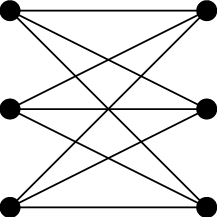
\includegraphics[scale=1]{bipartite_graph.png}
	\end{center}
	
	%		\item Vertices
	%		\begin{itemize}
	%			\item Sink $S$
	%			\item se
	%		\end{itemize}
	
\end{itemize}
\end{frame}

\begin{frame}{Sensors-Relays graph - Vertices}
\begin{itemize}
\item Number of Vertices = $M + N + 2$
\item Source $S$
\item Sensors $\{s_1, s_2, s_3, ..., s_N\}$
\end{itemize}

\begin{center}
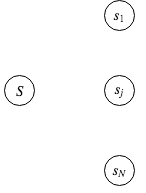
\includegraphics[scale=0.4]{sensors.png}
\end{center}
\end{frame}

\begin{frame}{Sensors-Relays graph - Vertices}
\begin{itemize}
%%	\item Number of Vertices = $M + N + 2$
\item Sink $F$
\item Possible locations $\{f_1, f_2, f_3,..., f_M\}$\\
\end{itemize}
\begin{center}
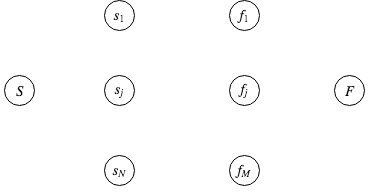
\includegraphics[scale=0.4]{sensors-relays.png}
\end{center}
\end{frame}

\begin{frame}{Sensors-Relays graph - Edge}
\begin{itemize}
\item Connected graph
\item The directions of all edges are from Source to Sink
\end{itemize}
\begin{center}
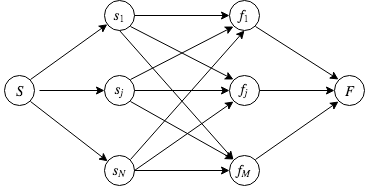
\includegraphics[scale=0.5]{connected.png}
\end{center}
\end{frame}

\begin{frame}{Sensors-Relays Graph - Flow}
\begin{itemize}
\item $capacity(S, s_i) = 1 ~ \forall ~ 0 < i \le N$
\item $capacity(s_i, f_j) = 1 ~  \forall ~ 0 < i \le N | 0 < j \le M$
\item $capacity(f_j, F) =  N/Y ~ \forall ~ 0 < j < M$
\end{itemize}

\begin{center}
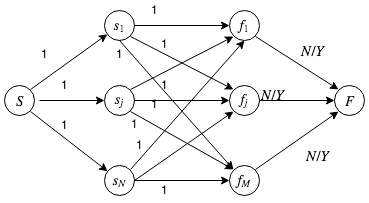
\includegraphics[scale=0.5]{flow_connected.png}
\end{center}
\end{frame}

\begin{frame}{Sensors-Relays Graph-Cost Flow}
\begin{itemize}
\item $cost(S, s_i) = 1 ~ \forall 0 < i < N$
\item $cost(s_i, f_j) = t_{s_i, f_j} ~ \forall 0 < i < N | 0 < j < M$
\item $cost(f_j, F) =  1$
\end{itemize}

\begin{center}
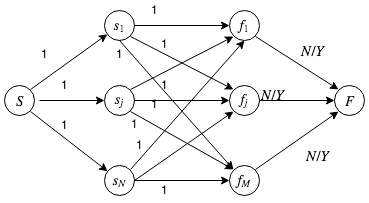
\includegraphics[scale=0.5]{flow_connected.png}

\end{center}
\end{frame}

\begin{frame}{Sensors-Relays Graph-Cost Flow}
\begin{itemize}
\item Characteristic
\begin{itemize}
\item $Y$ relays
\item $N$ sensors
\item each relay connect to $N/Y$ sensors
\end{itemize}
\item Optimal value of min-cost max-flow would give out the best solution for an individual
\end{itemize}
\end{frame}

\begin{frame}{Encoding Scheme}
	\begin{itemize}
		\item Individual
			\begin{itemize}
				\item Represents values for possible locations of relays and positions of relays
				\item $gen = \{0, 1\}$
				\item $gen = 1$ if this location will be placed by a relay
				\item $gen = 0$ if this location will not be placed by a relay
			\end{itemize}
		\item Example
	\end{itemize}
	\begin{center}
		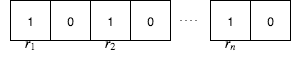
\includegraphics[scale=0.6]{encodeSchem2.png}
	\end{center}
\end{frame}


\begin{frame}{Fitness function}
	\begin{itemize}
		\item $capacity(f_j, F) = \begin{cases}
		N/Y ~ \text{If the $j$th location is chosen},\\
		0 ~ \text{If the $j$th location is not chosen}
		\end{cases}$
		\item Take the optimal value of min-cost maximum flow for the fitness value
%		\item $\{s_1, s_2, s_3, ..., s_n\}$ is the set of sensors
%		\item $\{f_1, f_2, f_3, ..., f_m\}$ is the set of possible relays
%		\item $s$ and $f$ is the simulated source and sink
		\item Example
	\end{itemize}
	\begin{center}
		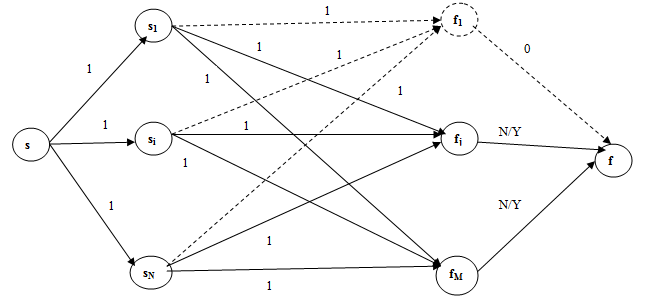
\includegraphics[scale=0.3]{max_flow3.png}
	\end{center}
\end{frame}



\begin{frame}{GA with Maximum Flow}
	\begin{itemize}
		\item Initialization
			\begin{itemize}
				\item Random initialization
				\item Normalize individual for ensuring the number of relays is $n$
			\end{itemize}
		\item Crossover
			\begin{itemize}
				\item Two point Crossover
			\end{itemize}
		\item Mutation
			\begin{itemize}
				\item Shuffle index mutation
				\item Probability $=0.2$
			\end{itemize}
		\item Selection
			\begin{itemize}
				\item Tournament selection
			\end{itemize}
	\end{itemize}
\end{frame}

\end{document}
